\documentclass[presentation]{beamer}
\mode<presentation>{\usetheme{AMSBolognaFCrev}}

\usepackage[utf8]{inputenc}
\usepackage[T1]{fontenc}
\usepackage{booktabs}
\usepackage{array}
\usepackage{colortbl}
\usepackage{tabularx}
\usepackage{tikz}
\usepackage{amsmath}
\usepackage[ddmmyyyy]{datetime}
\usepackage[export]{adjustbox}
\usetikzlibrary{arrows.meta,positioning,shapes.geometric,fit,calc}

\tikzset{
  lessonbox/.style={draw, rounded corners, align=center, font=\scriptsize,
    minimum height=0.68cm, text width=1.95cm},
  lessonarrow/.style={-{Stealth[length=2mm]}, thick}
}

\renewcommand{\dateseparator}{/}
\newcommand{\sectiontitleframe}[1]{
\begin{frame}[plain,c]
\begin{center}
{\usebeamerfont{title}\usebeamercolor[fg]{title}#1}
\end{center}
\end{frame}
}

\title[Lesson 5]{Authentication in Healthcare Systems}
\institute[Data Privacy and Security]{Healthcare Data Privacy and Security}
\author[\sspeaker{G. Pisano}]{\speaker{Giuseppe Pisano} \\\href{mailto:g.pisano@unibo.it}{g.pisano@unibo.it}}
\date[August, 2026]{August, 2026}
%
\titlegraphic{
\begin{center}
    
\includegraphics[width=0.35\textwidth, valign=c]{logos/intestazione.png}
    
\includegraphics[width=0.16\textwidth, valign=c]{logos/unibo_logo_2.png}
    
\includegraphics[width=0.11\textwidth, valign=c]{logos/makeni_logo_2.png}
    
\includegraphics[width=0.20\textwidth, valign=c]{logos/cuamm_logo_png.png}
\end{center}
\centering
\tiny{S.K.I.L.L.E.D --- AID013244/04/2\\Strategic Knowledge and Inclusive Lifelong Learning in the health sector for youth Employability and Development}
}

\newcommand{\scenario}{St. Isidore Hospital}
\newcommand{\takeawaysframe}[2]{
  \begin{frame}[c]{Recap: \insertsection}
    \begin{block}{What to keep}
      #1
    \end{block}
    \begin{exampleblock}{In \scenario}
      #2
    \end{exampleblock}
  \end{frame}
}

\begin{document}

\setbeamertemplate{frametitle}
{
    \nointerlineskip
    \begin{beamercolorbox}[sep=0.3cm,ht=2.2em,wd=\paperwidth]{frametitle}
        \vbox{}\vskip-2ex%
        \strut\insertframetitle\hfill\raisebox{-0.2\height}{
\includegraphics[width=2cm]{logos/cuamm_logo_png.png}}\strut
        \vskip-0.8ex%
    \end{beamercolorbox}
}

\begin{frame}[allowframebreaks]
  \titlepage
\end{frame}

\begin{frame}[c,allowframebreaks]{Roadmap}
\tableofcontents[hideallsubsections]
\end{frame}

\begin{frame}[c]{Running Scenario}
  Throughout the lesson we follow \textbf{\scenario}, a mid-size hospital with an electronic health record, a laboratory system, a pharmacy module, a patient portal, shared ward workstations, and remote access for clinicians on call.

  \begin{exampleblock}{The authentication question}
    Before the hospital can decide what a person may do, it must decide whether the person is really the doctor, nurse, pharmacist, patient, or administrator they claim to be.
  \end{exampleblock}
\end{frame}

\begin{frame}[c]{How This Lesson Progresses}
  \begin{enumerate}
    \item We start with the meaning of \textbf{authentication}: identity claims, identifiers, and verification.
    \item We classify authentication factors: \textit{knowledge}, \textit{possession}, \textit{inherence}, and \textit{behavior}.
    \item We study passwords as the most common mechanism, including hashes, salts, cracking, and policy.
    \item We move to physical and logical tokens, smart cards, and remote challenge-response.
    \item We finish with attacks, multi-factor authentication, one-time passwords, and modern phishing-resistant authenticators.
  \end{enumerate}
\end{frame}

\begin{frame}[c]{Connection with Other Lessons}
  Authentication connects several parts of the security architecture.

  \begin{block}{Relationship with earlier topics}
    \textbf{Access control} asks what an authenticated subject is allowed to do. Authentication asks whether the subject is really who they claim to be.
  \end{block}

  \begin{block}{Relationship with later topics}
    \textbf{Encryption} protects credentials and sessions in transit and at rest. \textbf{GDPR} requires appropriate security for personal data, which includes preventing unauthorized access to health records.
  \end{block}
\end{frame}

\section{Authentication Foundations}
\sectiontitleframe{Authentication Foundations}

\begin{frame}[c]{Section Context: Authentication Foundations}
\begin{block}{What we are talking about}
Authentication is the security function that connects an \textbf{identity claim} to evidence. It
comes before access control because the system cannot apply a policy to ``Dr. Moretti'' unless it
first verifies that the actor really is Dr. Moretti.
\end{block}

\begin{exampleblock}{Hospital lens}
At \scenario, the same foundation applies to staff logins, patient portal accounts, medical devices,
and service accounts used by applications.
\end{exampleblock}
\end{frame}

\begin{frame}[c]{Why Authentication Matters}
  Authentication is the process that verifies a claimed identity of, or for, a system \cite{rfc4949}. In practice, it is the first line of defense because every later control depends on it.

  \begin{exampleblock}{Hospital example}
    If someone opens the oncology record of patient Maria Rossi, the hospital needs more than ``a workstation did it.'' It needs to know whether the actor was Dr. Moretti, a ward nurse, a lab technician, or an attacker using an abandoned session.
  \end{exampleblock}

  \begin{block}{Core idea}
    Authentication creates accountability: actions can be linked to a verified identity, not merely to a device or network address.
  \end{block}
\end{frame}

\begin{frame}[c]{Identification and Verification}
  Authentication usually has two steps.

  \begin{block}{Identification}
    The subject presents an \textbf{identifier}: a username, badge ID, employee number, device name, API client ID, or patient portal account.
  \end{block}

  \begin{block}{Verification}
    The subject presents or generates \textbf{authentication information} that proves the identifier belongs to them: a password, PIN, token response, biometric sample, certificate signature, or OTP.
  \end{block}

  \begin{exampleblock}{Hospital example}
    The login name \texttt{l.bianchi} identifies a nurse. Her password and second factor verify that the person typing is likely Nurse Bianchi.
  \end{exampleblock}
\end{frame}

\begin{frame}[c]{Authentication Is Not Authorization}
  These terms are related, but they answer different questions.

  \begin{block}{Three questions}
    \textbf{Identification}: Who are you claiming to be?

    \textbf{Authentication}: Can you prove that claim?

    \textbf{Authorization}: Given that identity, what are you allowed to do?
  \end{block}

  \begin{exampleblock}{Hospital example}
    Dr. Moretti can authenticate successfully and still be denied access to payroll files. Authentication proves identity; it does not automatically grant every permission.
  \end{exampleblock}
\end{frame}

\begin{frame}[c]{User and Message Authentication}
  The word authentication appears in more than one context.

  \begin{block}{User authentication}
    The system validates the identity of a human or service account before allowing interaction.
  \end{block}

  \begin{block}{Message authentication}
    Communicating parties verify that a message was not altered and that it came from an authentic source.
  \end{block}

  \begin{exampleblock}{Hospital example}
    A doctor logging into the EHR needs user authentication. A lab result sent from the laboratory system to the EHR needs message authentication so the EHR can trust both the source and the content.
  \end{exampleblock}
\end{frame}

\begin{frame}[c]{Authentication Pipeline}
  \begin{center}
  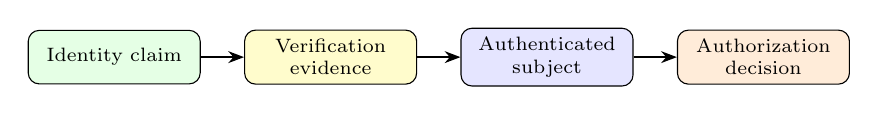
\begin{tikzpicture}[node distance=0.55cm]
    \node[lessonbox, fill=green!10] (claim) {Identity claim};
    \node[lessonbox, right=of claim, fill=yellow!20] (verify) {Verification evidence};
    \node[lessonbox, right=of verify, fill=blue!10] (subject) {Authenticated subject};
    \node[lessonbox, right=of subject, fill=orange!15] (access) {Authorization decision};
    \draw[lessonarrow] (claim) -- (verify);
    \draw[lessonarrow] (verify) -- (subject);
    \draw[lessonarrow] (subject) -- (access);
  \end{tikzpicture}
  \end{center}

  \vspace{0.5cm}
  \begin{exampleblock}{Hospital example}
    \texttt{m.rossi} plus valid authentication evidence becomes the authenticated subject ``Dr. Rossi.'' The access-control system can then evaluate whether Dr. Rossi may prescribe a controlled drug.
  \end{exampleblock}
\end{frame}

\takeawaysframe{
  Authentication binds a claimed identifier to evidence. It is different from authorization, but authorization depends on it. User authentication proves the actor; message authentication protects communication.
}{
  The hospital cannot safely enforce roles, audit accesses, or investigate incidents unless it can trust the identity attached to each action.
}

\section{Authentication Factors}
\sectiontitleframe{Authentication Factors}

\begin{frame}[c]{Section Context: Authentication Factors}
\begin{block}{What we are talking about}
Authentication mechanisms differ by the kind of evidence they request. Classifying factors helps us
understand why a password, a badge, a fingerprint, and a smart card do not fail in the same way.
\end{block}

\begin{exampleblock}{Hospital lens}
The hospital may use a password for the patient portal, a badge and PIN for medication cabinets,
and stronger MFA for remote EHR access.
\end{exampleblock}
\end{frame}

\begin{frame}[c]{Four Factor Families}
  Authentication factors are commonly grouped into four families.

  \begin{block}{Knowledge}
    Something the user \textbf{knows}: password, PIN, recovery phrase, or answer to a secret question.
  \end{block}

  \begin{block}{Possession}
    Something the user \textbf{has}: badge, smart card, hardware token, phone, cryptographic key, or authenticator app.
  \end{block}

  \begin{block}{Inherence and behavior}
    Something the user \textbf{is}: face or fingerprint. Something the user \textbf{does}: voice pattern, handwriting dynamics, or typing rhythm.
  \end{block}
\end{frame}

\begin{frame}[c]{Strengths and Weaknesses}
  No factor is perfect.

  \begin{block}{Knowledge factors}
    Passwords can be guessed, reused, phished, forgotten, or written down.
  \end{block}

  \begin{block}{Possession factors}
    Tokens can be lost, stolen, duplicated, damaged, or unavailable during emergencies.
  \end{block}

  \begin{block}{Biometrics}
    Biometrics can be convenient, but they raise false positive, false negative, privacy, cost, and recovery issues. A compromised password can be changed; a compromised fingerprint cannot be replaced in the same way.
  \end{block}
\end{frame}

\begin{frame}[c]{Running Example: Same Login, Different Factors}
  Imagine three ways to access the medication administration record.

  \begin{exampleblock}{Password only}
    Nurse Bianchi types a username and password on a shared ward workstation.
  \end{exampleblock}

  \begin{exampleblock}{Badge plus PIN}
    The workstation requires her hospital badge and a short PIN before opening the medication screen.
  \end{exampleblock}

  \begin{exampleblock}{Smart card plus biometric unlock}
    For high-risk actions, such as approving chemotherapy, the system requires a smart card unlocked locally with a fingerprint.
  \end{exampleblock}
\end{frame}

\begin{frame}[c]{Multi-Factor Authentication Principle}
  \begin{block}{Definition}
    Multi-factor authentication combines evidence from \textbf{different factor families}. A password plus another password is still knowledge-only; a password plus a smart card is multi-factor.
  \end{block}

  \begin{exampleblock}{Hospital example}
    Remote access to the EHR should not depend only on Dr. Moretti's password. A stolen password from a phishing email becomes less useful if the attacker also needs a hardware token or phishing-resistant authenticator.
  \end{exampleblock}
\end{frame}

\begin{frame}[c]{Scheme: Combining Factors}
  \begin{center}
  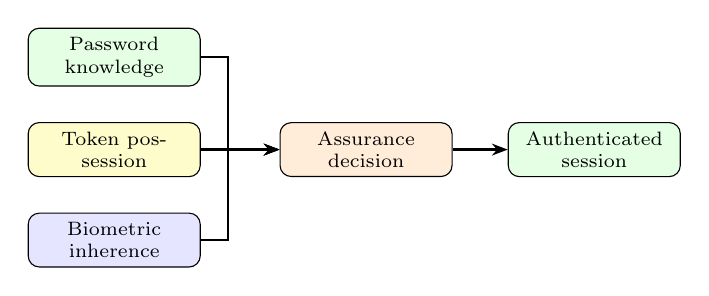
\begin{tikzpicture}[node distance=0.45cm]
    \node[lessonbox, fill=green!10] (p) {Password knowledge};
    \node[lessonbox, below=of p, fill=yellow!20] (t) {Token possession};
    \node[lessonbox, below=of t, fill=blue!10] (b) {Biometric inherence};
    \node[lessonbox, right=1.0cm of t, fill=orange!15] (d) {Assurance decision};
    \node[lessonbox, right=0.7cm of d, fill=green!10] (ok) {Authenticated session};
    \draw[lessonarrow] (p.east) -- ++(0.35,0) |- (d.west);
    \draw[lessonarrow] (t.east) -- (d.west);
    \draw[lessonarrow] (b.east) -- ++(0.35,0) |- (d.west);
    \draw[lessonarrow] (d) -- (ok);
  \end{tikzpicture}
  \end{center}

  \vspace{0.2cm}
  \begin{block}{Design point}
    More factors can increase assurance, but they also affect usability, recovery, support workload, and emergency access.
  \end{block}
\end{frame}

\takeawaysframe{
  Authentication factors are not interchangeable. Each factor family fails differently, so combining independent factors can reduce the chance that one compromise becomes full account access.
}{
  Password-only access may be acceptable for low-risk internal systems, but remote EHR access and high-impact clinical actions need stronger assurance.
}

\section{Passwords and Password Files}
\sectiontitleframe{Passwords and Password Files}

\begin{frame}[c]{Section Context: Passwords and Password Files}
\begin{block}{What we are talking about}
Passwords are still the most common authentication mechanism. The security question is not only
whether users choose good passwords, but also how the system stores, verifies, protects, and monitors
password-derived data.
\end{block}

\begin{exampleblock}{Hospital lens}
If the EHR password database is stolen, the difference between plaintext passwords and salted slow
hashes may decide whether the incident becomes a hospital-wide account compromise.
\end{exampleblock}
\end{frame}

\begin{frame}[c]{Password-Based Authentication}
  In a password system, the password verifies the user ID.

  \begin{block}{What the user ID does}
    It determines whether the account exists, which privileges are attached to it, and how the system refers to the user in access-control rules and logs.
  \end{block}

  \begin{block}{What the password does}
    It provides evidence that the person using that user ID is the legitimate account holder.
  \end{block}

  \begin{exampleblock}{Hospital example}
    The user ID \texttt{pharma.galli} links to pharmacy privileges. The password is supposed to prevent a different employee from using those privileges.
  \end{exampleblock}
\end{frame}

\begin{frame}[c]{Password Files Store Verifiers}
  A well-designed system should not store plaintext passwords.

  \begin{block}{Stored verifier}
    The system stores a value derived from the password using a one-way password hashing function. During login, the system recomputes the verifier from the submitted password and compares it with the stored value.
  \end{block}

  \begin{exampleblock}{Hospital example}
    If the EHR database is copied during an incident, plaintext passwords would immediately endanger every clinician account. Password hashes limit the damage, although weak passwords may still be cracked offline.
  \end{exampleblock}
\end{frame}

\begin{frame}[c]{Scheme: Password Verification}
  \begin{center}
  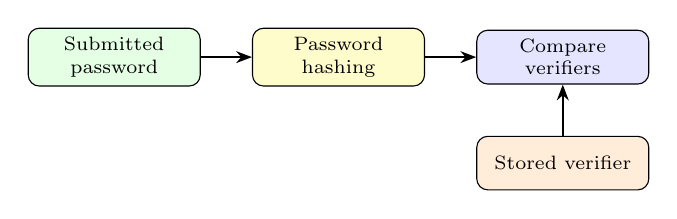
\begin{tikzpicture}[node distance=0.65cm]
    \node[lessonbox, fill=green!10] (input) {Submitted password};
    \node[lessonbox, right=of input, fill=yellow!20] (hash) {Password hashing};
    \node[lessonbox, right=of hash, fill=blue!10] (compare) {Compare verifiers};
    \node[lessonbox, below=of compare, fill=orange!15] (db) {Stored verifier};
    \draw[lessonarrow] (input) -- (hash);
    \draw[lessonarrow] (hash) -- (compare);
    \draw[lessonarrow] (db) -- (compare);
  \end{tikzpicture}
  \end{center}

  \vspace{0.5cm}
  \begin{block}{Important}
    Hashing is not encryption. There should be no decryption key that recovers the original password.
  \end{block}
\end{frame}

\begin{frame}[c]{Common Password Attacks}
  \small
  \begin{tabularx}{\textwidth}{@{}p{0.28\textwidth}X@{}}
    \toprule
    \textbf{Attack} & \textbf{Hospital example} \\
    \midrule
    Offline dictionary attack & An attacker steals password hashes from an old backup and tests likely passwords on their own machine. \\
    Specific account attack & A former contractor repeatedly tries to guess the head nurse's password. \\
    Popular password attack & The attacker tries \texttt{Password123!}, season names, and hospital-themed passwords across many accounts. \\
    Workstation hijacking & Someone uses a workstation where a clinician walked away without locking the session. \\
    Password reuse & A password leaked from a personal site is reused for the patient portal. \\
    Electronic monitoring & A keylogger captures credentials typed on a compromised endpoint. \\
    \bottomrule
  \end{tabularx}
\end{frame}

\begin{frame}[c]{Countermeasures Are Layered}
  \begin{block}{Prevent guessing}
    Use minimum length, block known compromised passwords, avoid predictable composition rules, and rate-limit online attempts \cite{nist80063b4}.
  \end{block}

  \begin{block}{Reduce value of stolen files}
    Protect password databases, use salted slow password hashes, restrict backups, monitor access, and force resets after confirmed compromise.
  \end{block}

  \begin{block}{Protect active sessions}
    Use workstation locking, inactivity timeouts, reauthentication for sensitive actions, and strong session management.
  \end{block}
\end{frame}

\begin{frame}[c]{Salted Password Hashes}
  A \textbf{salt} is a random value stored with a password verifier.

  \begin{block}{How it works}
    When a password is created, the system generates a unique salt, combines it with the password, and computes a password hash. The stored record contains the salt and the resulting verifier.
  \end{block}

  \begin{exampleblock}{Hospital example}
    If two nurses choose the same password, their stored hashes should still be different. Otherwise, an attacker can immediately see password reuse inside the hospital.
  \end{exampleblock}
\end{frame}

\begin{frame}[c]{Scheme: Salted Password Storage}
  \begin{center}
  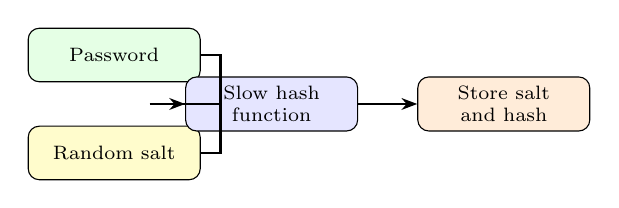
\begin{tikzpicture}[node distance=0.55cm]
    \node[lessonbox, fill=green!10] (pw) {Password};
    \node[lessonbox, below=of pw, fill=yellow!20] (salt) {Random salt};
    \coordinate[right=0.45cm of $(pw)!0.5!(salt)$] (join);
    \node[lessonbox, right=0.45cm of join, fill=blue!10] (hash) {Slow hash function};
    \node[lessonbox, right=0.75cm of hash, fill=orange!15] (db) {Store salt and hash};
    \draw[thick] (pw.east) -- ++(0.25,0) |- (join);
    \draw[thick] (salt.east) -- ++(0.25,0) |- (join);
    \draw[lessonarrow] (join) -- (hash.west);
    \draw[lessonarrow] (hash) -- (db);
  \end{tikzpicture}
  \end{center}

  \vspace{0.45cm}
  \begin{block}{Security effect}
    Salts make duplicate passwords less visible and make precomputed rainbow tables much less useful.
  \end{block}
\end{frame}

\begin{frame}[c]{Why Salt Helps Against Cracking}
  \begin{block}{Without salt}
    An attacker can compute a large table of password hashes once and reuse it against many systems.
  \end{block}

  \begin{block}{With salt}
    The attacker must test candidate passwords together with each account's salt. The same password produces different stored values across users and systems.
  \end{block}

  \begin{exampleblock}{Hospital example}
    A stolen radiology application backup contains salted hashes. The attacker can still try guesses, but cannot simply use a generic table of common password hashes.
  \end{exampleblock}
\end{frame}

\begin{frame}[c]{Historical UNIX Password Schemes}
  \small
  \begin{tabularx}{\textwidth}{@{}p{0.25\textwidth}X@{}}
    \toprule
    \textbf{Scheme} & \textbf{What it teaches} \\
    \midrule
    Original \texttt{crypt(3)} & DES-based, short password limit, small salt, repeated computation. Historically important, but obsolete for modern systems. \\
    MD5 and SHA-based schemes & Longer passwords and more iterations, but MD5 is obsolete and simple fast hashes are not appropriate for password storage. \\
    bcrypt & Uses a salt and a variable work factor so administrators can make cracking more expensive as hardware improves. \\
    \bottomrule
  \end{tabularx}

  \begin{block}{Modern note}
    Current systems should use password hashing functions designed for passwords, such as \textbf{bcrypt}, \textbf{scrypt}, \textbf{Argon2}, or platform-approved equivalents.
  \end{block}
\end{frame}

\begin{frame}[c]{Password Cracking}
  Password cracking rarely tries every possible string first. It exploits human choices.

  \begin{block}{Dictionary and mutation attacks}
    Attackers start from common passwords, names, places, dates, keyboard patterns, and leaked password lists. Then they mutate them with uppercase letters, numbers, symbols, reversals, and substitutions.
  \end{block}

  \begin{exampleblock}{Hospital example}
    \texttt{StIsidore2026!} looks complex, but it is built from public information and a year. A hospital-themed password is exactly the kind of candidate an attacker would try.
  \end{exampleblock}
\end{frame}

\begin{frame}[c]{Rainbow Tables}
  \begin{block}{Idea}
    A rainbow table trades storage for speed. Instead of hashing guesses during the attack, the attacker prepares large sets of password-hash relationships in advance.
  \end{block}

  \begin{block}{Limits}
    Long salts and slow password hashing functions make generic precomputation much less useful. The attacker must do more account-specific work.
  \end{block}

  \begin{exampleblock}{Hospital example}
    If an old departmental application stores unsalted MD5 password hashes, a public rainbow table may reveal many passwords quickly. If it stores salted bcrypt hashes, the attack becomes much more expensive.
  \end{exampleblock}
\end{frame}

\begin{frame}[c]{Shadow Password Files}
  Shadow password files separate public account information from protected password verifiers.

  \begin{block}{Purpose}
    Normal users may need to read account names or user IDs, but they should not read password hashes. Shadow files restrict hash access to privileged components.
  \end{block}

  \begin{block}{Residual risks}
    Operating-system vulnerabilities, permission mistakes, weak backup protection, password reuse, and network sniffing can still expose credentials or usable authentication data.
  \end{block}
\end{frame}

\takeawaysframe{
  Password systems depend on careful verifier storage, salts, slow hashing, rate limits, protected backups, and session controls. A hash leak is not harmless; it starts an offline race between attacker guesses and defensive design.
}{
  The hospital should assume some passwords will be weak or reused, so password security must include technical controls, monitoring, and MFA for sensitive systems.
}

\section{Password Policy}
\sectiontitleframe{Password Policy}

\begin{frame}[c]{Section Context: Password Policy}
\begin{block}{What we are talking about}
Password policy shapes user behavior. A policy that looks strict on paper can be weak in practice
if it encourages predictable choices, password reuse, or written notes.
\end{block}

\begin{exampleblock}{Hospital lens}
Clinical staff authenticate under time pressure. The policy must protect patients without making
legitimate care workflows unnecessarily difficult.
\end{exampleblock}
\end{frame}

\begin{frame}[c]{The Policy Tension}
  Password policy must balance two goals.

  \begin{block}{Security goal}
    Eliminate passwords that are easy to guess, reuse, or find in breach lists.
  \end{block}

  \begin{block}{Usability goal}
    Allow users to choose secrets they can remember without writing them on a monitor, sharing them with colleagues, or using predictable transformations.
  \end{block}

  \begin{exampleblock}{Hospital example}
    A nurse moving between patients cannot safely manage a password rule that changes every month and requires obscure symbols. Bad usability becomes a security risk.
  \end{exampleblock}
\end{frame}

\begin{frame}[c]{User Education and Passphrases}
  Education alone is not sufficient, but it helps users understand what the policy is trying to prevent.

  \begin{block}{Passphrase approach}
    A memorable sentence can be transformed into a longer secret. Length usually matters more than decorative complexity, provided the phrase is not obvious or reused.
  \end{block}

  \begin{exampleblock}{Hospital example}
    A clinician might build a private passphrase from a personal sentence, not from the hospital name, ward name, favorite team, date of birth, or medical specialty.
  \end{exampleblock}
\end{frame}

\begin{frame}[c]{Generated Passwords and Password Managers}
  Computer-generated passwords can be strong, but only if users have a usable way to store and use them.

  \begin{block}{Random generation}
    Random long passwords are difficult to guess but hard to memorize.
  \end{block}

  \begin{block}{Password managers}
    A managed password vault can generate unique passwords for many systems, reducing reuse. In a hospital, this must be aligned with endpoint security, recovery procedures, and emergency access rules.
  \end{block}
\end{frame}

\begin{frame}[c]{Reactive Password Checking}
  \begin{block}{Method}
    The organization periodically runs a password cracker against its own password hashes to find weak passwords.
  \end{block}

  \begin{block}{Problem}
    The weak password remains valid until the check finds it. The process also consumes resources and requires very careful handling of password hashes.
  \end{block}

  \begin{exampleblock}{Hospital example}
    Security staff discover that several accounts use passwords based on ward names. Those users are forced to reset passwords, but the accounts were exposed before discovery.
  \end{exampleblock}
\end{frame}

\begin{frame}[c]{Proactive Password Checking}
  \begin{block}{Method}
    The system checks password quality at creation time and rejects weak choices before they become active.
  \end{block}

  \begin{block}{Modern checks}
    Useful checks include minimum length, known-compromised password lists, blocklists of local terms, and detection of obvious patterns. Overly rigid composition rules can backfire.
  \end{block}

  \begin{exampleblock}{Hospital example}
    The patient portal rejects \texttt{StIsidore2026!} because it contains the hospital name and a predictable year, even though it contains uppercase, lowercase, digits, and punctuation.
  \end{exampleblock}
\end{frame}

\begin{frame}[c]{Lockout, Rate Limits, and Availability}
  Account lockout can slow guessing, but it can also be abused.

  \begin{block}{Lockout risk}
    An attacker may intentionally fail login attempts for the emergency department director and lock the account during a crisis.
  \end{block}

  \begin{block}{Balanced design}
    Use rate limits, risk-based throttling, alerting, step-up authentication, and recovery paths that preserve clinical continuity without allowing easy bypass.
  \end{block}
\end{frame}

\takeawaysframe{
  Password policy should prevent weak choices at creation, limit online guessing, avoid unnecessary user burden, and support safe recovery. The goal is not theatrical complexity; it is resistance to realistic attacks.
}{
  A hospital password policy must work during a busy shift. If users cannot follow it, they will invent workarounds that weaken authentication.
}

\section{Tokens and Smart Cards}
\sectiontitleframe{Tokens and Smart Cards}

\begin{frame}[c]{Section Context: Tokens and Smart Cards}
\begin{block}{What we are talking about}
Possession factors add something the user has to the authentication process. Tokens can be simple
storage objects, cryptographic devices, smart cards, phones, or hardware security keys.
\end{block}

\begin{exampleblock}{Hospital lens}
A staff badge can unlock a door, but a smart card can also prove possession of a protected key
during workstation or application login.
\end{exampleblock}
\end{frame}

\begin{frame}[c]{What Is a Token?}
  A token is a physical or logical object possessed by the user and used during authentication.

  \begin{block}{Common examples}
    Badge cards, magnetic stripe cards, memory cards, smart cards, hardware security keys, authenticator apps, and software certificates.
  \end{block}

  \begin{exampleblock}{Hospital example}
    A staff badge can open doors. A smart card can also participate in computer login by proving possession of a cryptographic secret.
  \end{exampleblock}
\end{frame}

\begin{frame}[c]{Card Types}
  \small
  \begin{tabularx}{\textwidth}{@{}p{0.24\textwidth}X@{}}
    \toprule
    \textbf{Type} & \textbf{Authentication meaning} \\
    \midrule
    Embossed card & Carries visible identity information; weak as a digital authenticator. \\
    Magnetic stripe & Stores simple data that can often be read or copied by compatible readers. \\
    Memory card & Stores data electronically but does not process it securely. \\
    Smart card & Includes processing capability and can execute authentication protocols. \\
    Contact card & Communicates through exposed electrical contacts. \\
    Contactless card & Communicates through a radio interface. \\
    \bottomrule
  \end{tabularx}
\end{frame}

\begin{frame}[c]{Memory Cards}
  \begin{block}{Capability}
    Memory cards can store information but do not independently process secrets or run cryptographic protocols.
  \end{block}

  \begin{block}{Security model}
    They are often combined with a PIN. The attacker needs both the card and the PIN, which is stronger than a password alone.
  \end{block}

  \begin{exampleblock}{Hospital example}
    A badge plus PIN may unlock a medication cabinet. If the badge is stolen, the PIN still matters; if the PIN is observed, the badge still matters.
  \end{exampleblock}
\end{frame}

\begin{frame}[c]{Memory Card Limitations}
  \begin{block}{Reader dependency}
    Special readers increase cost and must themselves be protected.
  \end{block}

  \begin{block}{Loss and replacement}
    Lost tokens interrupt work and require revocation, replacement, and sometimes identity re-verification.
  \end{block}

  \begin{block}{User acceptance}
    A token used once a day may be accepted. A token required dozens of times per shift may create fatigue unless workflows are designed carefully.
  \end{block}
\end{frame}

\begin{frame}[c]{Smart Cards}
  Smart cards are more capable than memory cards because they contain a microprocessor and memory.

  \begin{block}{Internal components}
    A smart card can include ROM for permanent data, EEPROM for applications and changing state, RAM for temporary data, I/O interfaces, and sometimes cryptographic acceleration.
  \end{block}

  \begin{exampleblock}{Hospital example}
    A clinician smart card can store or protect a private key. During login, the card proves possession of that key without revealing it to the workstation.
  \end{exampleblock}
\end{frame}

\begin{frame}[c]{Smart Card Authentication Protocols}
  \begin{block}{Static}
    The card presents a fixed credential after the user unlocks it. This is simple but weaker if the credential can be copied.
  \end{block}

  \begin{block}{Dynamic password generator}
    The card generates changing codes. The verifier accepts a code only if it matches the expected value for that moment or counter.
  \end{block}

  \begin{block}{Challenge-response}
    The system sends a fresh challenge. The card computes a response using a protected secret or private key.
  \end{block}
\end{frame}

\begin{frame}[c]{Scheme: Token Plus PIN}
  \begin{center}
  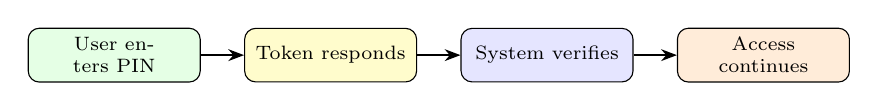
\begin{tikzpicture}[node distance=0.55cm]
    \node[lessonbox, fill=green!10] (pin) {User enters PIN};
    \node[lessonbox, right=of pin, fill=yellow!20] (token) {Token responds};
    \node[lessonbox, right=of token, fill=blue!10] (system) {System verifies};
    \node[lessonbox, right=of system, fill=orange!15] (ok) {Access continues};
    \draw[lessonarrow] (pin) -- (token);
    \draw[lessonarrow] (token) -- (system);
    \draw[lessonarrow] (system) -- (ok);
  \end{tikzpicture}
  \end{center}

  \vspace{0.45cm}
  \begin{exampleblock}{Hospital example}
    For controlled-drug dispensing, the cabinet requires the nurse's badge and PIN before logging the withdrawal under her identity.
  \end{exampleblock}
\end{frame}

\takeawaysframe{
  Tokens strengthen authentication because attackers must compromise something the user possesses, not only something the user knows. Smart cards can protect secrets and participate in cryptographic protocols.
}{
  Badge workflows can improve security, but the hospital must manage readers, lost tokens, revocation, replacement, and user fatigue.
}

\section{Remote Authentication}
\sectiontitleframe{Remote Authentication}

\begin{frame}[c]{Section Context: Remote Authentication}
\begin{block}{What we are talking about}
Remote authentication must cross a network, so the design must consider interception, replay,
phishing, fake endpoints, and compromised home devices.
\end{block}

\begin{exampleblock}{Hospital lens}
When a clinician connects from home, the hospital is no longer protecting only a local workstation.
It is protecting an authentication exchange across networks it does not fully control.
\end{exampleblock}
\end{frame}

\begin{frame}[c]{Local vs Remote Authentication}
  \begin{block}{Local authentication}
    The user authenticates to a nearby system, such as a workstation, local terminal, or ATM-like device.
  \end{block}

  \begin{block}{Remote authentication}
    Authentication data travels over a network. Attackers may observe traffic, replay old exchanges, or trick users into authenticating to a fake endpoint.
  \end{block}

  \begin{exampleblock}{Hospital example}
    A doctor logging in from a ward workstation faces local session risks. A doctor connecting from home to the EHR also faces network interception, phishing, and endpoint compromise risks.
  \end{exampleblock}
\end{frame}

\begin{frame}[c]{Replay Attacks}
  A replay attack reuses previously captured authentication data.

  \begin{block}{Problem}
    If the same password-derived response is valid every time, an attacker who records it once may use it later.
  \end{block}

  \begin{exampleblock}{Hospital example}
    An attacker monitoring a poorly protected remote login captures a valid authentication exchange from Dr. Moretti and later sends the same response to the VPN gateway.
  \end{exampleblock}
\end{frame}

\begin{frame}[c]{Challenge-Response Authentication}
  Challenge-response avoids sending a reusable secret.

  \begin{block}{Algorithm}
    The server sends a fresh random value called a \textbf{nonce}. The client computes a response using the nonce and a secret-derived value. The server checks whether the response is correct for that nonce.
  \end{block}

  \begin{block}{Security intuition}
    Because the nonce changes every time, yesterday's valid response should not authenticate today's login.
  \end{block}
\end{frame}

\begin{frame}[c]{Scheme: Challenge-Response}
  \begin{center}
  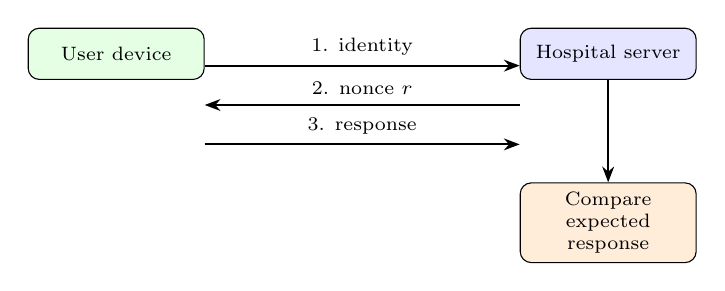
\begin{tikzpicture}[
    actor/.style={draw, rounded corners, align=center, font=\scriptsize,
      minimum height=0.65cm, text width=2.0cm},
    msg/.style={-{Stealth[length=2mm]}, thick},
    every node/.style={font=\scriptsize}
  ]
    \node[actor, fill=green!10] (u) {User device};
    \node[actor, right=4.0cm of u, fill=blue!10] (s) {Hospital server};
    \draw[msg] ($(u.east)+(0,-0.15)$) -- node[above]{1. identity} ($(s.west)+(0,-0.15)$);
    \draw[msg] ($(s.west)+(0,-0.65)$) -- node[above]{2. nonce $r$} ($(u.east)+(0,-0.65)$);
    \draw[msg] ($(u.east)+(0,-1.15)$) -- node[above]{3. response} ($(s.west)+(0,-1.15)$);
    \node[actor, below=1.3cm of s, fill=orange!15] (check) {Compare expected response};
    \draw[msg] (s) -- (check);
  \end{tikzpicture}
  \end{center}

  \vspace{0.45cm}
  \begin{block}{What is protected}
    The password and its direct hash are not sent as reusable network messages.
  \end{block}
\end{frame}

\begin{frame}[c]{Challenge-Response in the Hospital}
  \begin{exampleblock}{Remote EHR access}
    The VPN gateway stores a verifier for Dr. Moretti. At login, it sends a nonce. Dr. Moretti's client computes a response using the nonce and the secret-derived value. A captured response is useless for the next nonce.
  \end{exampleblock}

  \begin{block}{Important limit}
    Challenge-response protects against simple replay, but it does not automatically solve phishing, malware on the endpoint, stolen devices, weak recovery, or poor server validation.
  \end{block}
\end{frame}

\takeawaysframe{
  Remote authentication must avoid reusable secrets on the network. Nonces and challenge-response protocols make captured authentication exchanges less useful.
}{
  The hospital should treat remote access as higher risk than local access and require mechanisms that resist interception and replay.
}

\section{Attacks Against Authentication}
\sectiontitleframe{Attacks Against Authentication}

\begin{frame}[c]{Section Context: Attacks Against Authentication}
\begin{block}{What we are talking about}
Authentication can fail because a secret is guessed, a verifier database is stolen, a token is lost,
a fake interface captures credentials, or a legitimate user is locked out.
\end{block}

\begin{exampleblock}{Hospital lens}
For a hospital, authentication attacks are not only privacy incidents. They can interrupt care,
misattribute clinical actions, or allow unsafe changes to patient data.
\end{exampleblock}
\end{frame}

\begin{frame}[c]{Client-Side Attacks}
  \begin{block}{Guessing}
    The attacker tries to authenticate without compromising the server or network. Rate limits, throttling, lockout design, and strong password policy reduce feasibility.
  \end{block}

  \begin{block}{Token theft}
    If the system uses tokens, the attacker may need both the token and its activation factor, such as a PIN or biometric unlock.
  \end{block}

  \begin{exampleblock}{Hospital example}
    A stolen badge should not be enough to open the EHR. The badge must be revoked quickly and should require an additional factor for sensitive systems.
  \end{exampleblock}
\end{frame}

\begin{frame}[c]{Host-Side Attacks}
  \begin{block}{Credential verifier theft}
    The attacker obtains password hashes, token seeds, passcodes, certificates, or biometric templates from the authentication server.
  \end{block}

  \begin{block}{Defensive direction}
    Store only what is necessary, protect authenticators with strong access controls, use hardware security modules where appropriate, monitor privileged access, and avoid plaintext shared secrets.
  \end{block}

  \begin{exampleblock}{Hospital example}
    If the MFA seed database for staff tokens is exposed, attackers may generate valid OTPs. The authentication server is therefore a high-value clinical security asset.
  \end{exampleblock}
\end{frame}

\begin{frame}[c]{Interception and Observation}
  \begin{block}{Physical observation}
    Shoulder surfing, written passwords, badge sharing, and unattended sessions can bypass otherwise strong controls.
  \end{block}

  \begin{block}{Endpoint observation}
    Keyloggers, screen capture tools, malicious browser extensions, and compromised mobile devices can capture credentials or OTPs.
  \end{block}

  \begin{exampleblock}{Hospital example}
    A shared workstation in a busy ward is a high-risk environment. Screen privacy, automatic lock, fast reauthentication, and user training all matter.
  \end{exampleblock}
\end{frame}

\begin{frame}[c]{Trojan Horse Attacks}
  \begin{block}{Idea}
    A fake application or device presents itself as legitimate and captures credentials.
  \end{block}

  \begin{exampleblock}{Hospital example}
    A fake ``EHR password reset'' page sent by email asks Dr. Moretti for username, password, and OTP. If the attacker relays those values immediately, ordinary OTP MFA may still fail.
  \end{exampleblock}

  \begin{block}{Mitigation}
    Use phishing-resistant authenticators when possible, train users on expected flows, validate domains, and monitor suspicious authentication patterns.
  \end{block}
\end{frame}

\begin{frame}[c]{Denial of Service}
  Authentication can also be attacked by making legitimate login difficult or impossible.

  \begin{block}{System-wide DoS}
    The attacker floods the authentication service so staff cannot log in.
  \end{block}

  \begin{block}{Targeted lockout}
    The attacker intentionally fails logins for a specific account until it is locked.
  \end{block}

  \begin{exampleblock}{Hospital example}
    Locking the emergency physician's account during night shift may be as damaging as stealing it. Availability is part of authentication design.
  \end{exampleblock}
\end{frame}

\begin{frame}[c]{Attack Summary}
  \small
  \begin{tabularx}{\textwidth}{@{}p{0.23\textwidth}p{0.36\textwidth}X@{}}
    \toprule
    \textbf{Attack} & \textbf{What fails} & \textbf{Typical defenses} \\
    \midrule
    Guessing & Weak secrets and unlimited attempts & Rate limits, blocklists, MFA \\
    Host theft & Poorly protected verifier stores & Least privilege, slow hashes, HSMs, monitoring \\
    Interception & Reusable credentials or weak endpoint & TLS, challenge-response, endpoint hardening \\
    Replay & Static responses & Nonces, OTP, mutual authentication \\
    Trojan horse & User trusts fake interface & Phishing-resistant MFA, user training, monitoring \\
    DoS & Availability of login path & Throttling, resilient design, emergency access \\
    \bottomrule
  \end{tabularx}
\end{frame}

\takeawaysframe{
  Authentication attacks target people, endpoints, servers, networks, and recovery processes. A strong mechanism can still fail if the surrounding workflow is weak.
}{
  The hospital must protect both credential storage and everyday clinical authentication paths, especially shared workstations and remote access.
}

\section{Multi-Factor and One-Time Passwords}
\sectiontitleframe{Multi-Factor and One-Time Passwords}

\begin{frame}[c]{Section Context: Multi-Factor and One-Time Passwords}
\begin{block}{What we are talking about}
Multi-factor authentication reduces dependence on one credential. One-time passwords are a common
second factor, but they introduce secrets, time windows, enrollment, recovery, and phishing risks.
\end{block}

\begin{exampleblock}{Hospital lens}
The hospital may accept TOTP for ordinary remote login while requiring phishing-resistant
authenticators for administrators and other high-impact accounts.
\end{exampleblock}
\end{frame}

\begin{frame}[c]{Two-Step Authentication}
  In many systems, users first enter a password and then provide a second value generated by a token or app.

  \begin{block}{Common pattern}
    \textbf{First factor}: username and password.

    \textbf{Second factor}: one-time password, push approval, hardware token touch, smart-card response, or platform authenticator.
  \end{block}

  \begin{exampleblock}{Hospital example}
    A clinician logs into the remote access portal with username and password, then enters a six-digit code from an authenticator app.
  \end{exampleblock}
\end{frame}

\begin{frame}[c]{HOTP and TOTP}
  One-time passwords are usually generated from a shared secret and a changing value.

  \begin{block}{HOTP}
    HMAC-based OTP uses a counter. The token and server must agree on the counter value \cite{rfc4226}.
  \end{block}

  \begin{block}{TOTP}
    Time-based OTP replaces the counter with time steps. RFC 6238 defines TOTP as HOTP computed over a time value, commonly using 30-second windows \cite{rfc6238}.
  \end{block}
\end{frame}

\begin{frame}[c]{TOTP Enrollment}
  \begin{block}{Shared secret}
    During enrollment, the server creates a unique secret for the user. The user's app stores the same secret, often transferred through a QR code.
  \end{block}

  \begin{block}{Synchronization}
    The app and server must share a compatible algorithm and a sufficiently synchronized notion of time. Network Time Protocol helps systems maintain accurate time.
  \end{block}

  \begin{exampleblock}{Hospital example}
    Dr. Moretti scans a QR code into the authenticator app. From then on, the app and hospital server can generate matching codes for the same time window.
  \end{exampleblock}
\end{frame}

\begin{frame}[c]{Scheme: TOTP Login}
  \begin{center}
  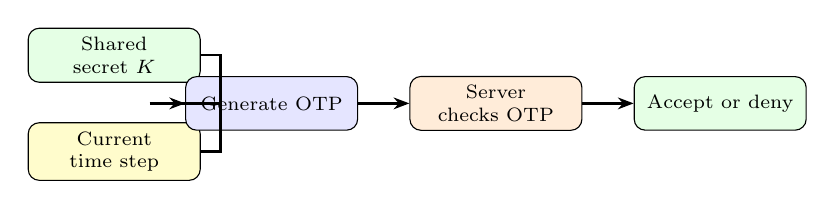
\begin{tikzpicture}[node distance=0.5cm]
    \node[lessonbox, fill=green!10] (secret1) {Shared secret $K$};
    \node[lessonbox, below=of secret1, fill=yellow!20] (time1) {Current time step};
    \coordinate[right=0.45cm of $(secret1)!0.5!(time1)$] (join);
    \node[lessonbox, right=0.45cm of join, fill=blue!10] (code1) {Generate OTP};
    \node[lessonbox, right=0.65cm of code1, fill=orange!15] (server) {Server checks OTP};
    \node[lessonbox, right=0.65cm of server, fill=green!10] (decision) {Accept or deny};
    \draw[thick] (secret1.east) -- ++(0.25,0) |- (join);
    \draw[thick] (time1.east) -- ++(0.25,0) |- (join);
    \draw[lessonarrow] (join) -- (code1.west);
    \draw[lessonarrow] (code1) -- (server);
    \draw[lessonarrow] (server) -- (decision);
  \end{tikzpicture}
  \end{center}

  \vspace{0.4cm}
  \begin{block}{Validity window}
    Servers often accept a small time window around the current step to tolerate clock drift and network delay.
  \end{block}
\end{frame}

\begin{frame}[c]{OTP Risks}
  \begin{block}{Physical or logical token compromise}
    If the phone, app storage, or token seed is compromised, the attacker may generate valid codes.
  \end{block}

  \begin{block}{Time-window attack}
    A captured OTP may be usable briefly. Real-time phishing can exploit this by relaying the code immediately.
  \end{block}

  \begin{block}{Migration and recovery}
    Replacing a phone is operationally sensitive because secrets must be re-bound or migrated safely.
  \end{block}
\end{frame}

\begin{frame}[c]{Same-Channel Problem}
  Two factors are stronger when they are independent. In practice, many factors meet on the same endpoint.

  \begin{block}{Problem}
    A user may type password and OTP into the same browser, with the same keyboard, on the same operating system. If that endpoint is compromised, both factors can be captured.
  \end{block}

  \begin{exampleblock}{Hospital example}
    Malware on a home laptop can capture the VPN password and TOTP code during the same login. MFA still helps, but endpoint security remains essential.
  \end{exampleblock}
\end{frame}

\begin{frame}[c]{Phishing-Resistant MFA}
  Some authenticators are designed to resist credential replay and phishing better than OTP.

  \begin{block}{Cryptographic authenticators}
    FIDO2/passkey-style authenticators use public-key cryptography and bind authentication to the legitimate service origin, making simple fake-site replay much harder \cite{fido2,nist80063b4}.
  \end{block}

  \begin{exampleblock}{Hospital example}
    For remote administrator access, the hospital may require a hardware security key. The key signs a challenge for the real hospital domain and does not reveal a reusable code to a fake page.
  \end{exampleblock}
\end{frame}

\takeawaysframe{
  MFA improves authentication by combining factors, but OTP is not magic. Shared secrets, time synchronization, recovery, phishing, and endpoint compromise all remain design concerns.
}{
  The hospital can use OTP for many staff workflows, but should prefer phishing-resistant MFA for remote access, administrators, and high-impact clinical systems.
}

\section{Authentication Lab}
\sectiontitleframe{Authentication Lab}

\begin{frame}[c]{Section Context: Authentication Lab}
\begin{block}{What we are talking about}
The lab turns the authentication mechanisms into small executable models. The goal is to see the
logic of password verifiers, replay resistance, and TOTP MFA without pretending that a notebook is a
production identity system.
\end{block}

\begin{exampleblock}{Hospital lens}
St. Isidore Hospital uses these examples to reason about policy choices. In real deployments,
administrators configure identity providers, MFA platforms, operating-system authentication,
logging, and recovery workflows.
\end{exampleblock}
\end{frame}

\begin{frame}[c]{Lab Setup}
\begin{block}{Environment}
Use the lesson-local virtual environment:
\texttt{lesson-05/.venv}
\end{block}

\begin{block}{Notebooks}
Open the notebooks in \texttt{lesson-05/examples} and select the \texttt{lesson-05/.venv} Python
kernel.
\end{block}

\begin{exampleblock}{Safety}
The examples use artificial users and toy policies only. Do not use real patient data, real staff
credentials, or production authentication secrets.
\end{exampleblock}
\end{frame}

\begin{frame}[c]{Notebook 1: Password Storage and Cracking}
\begin{block}{Open}
\texttt{lesson-05/examples/01\_password\_storage\_and\_cracking.ipynb}
\end{block}

\begin{block}{What it shows}
The notebook compares plaintext password storage with salted PBKDF2 verifiers, then simulates a
small offline dictionary attack against weak hospital-themed passwords.
\end{block}

\begin{exampleblock}{Running example}
Some St. Isidore accounts use predictable passwords such as hospital names, departments, or birth
years. The attacker does not need the real login page once the verifier file is stolen.
\end{exampleblock}
\end{frame}

\begin{frame}[c]{Notebook 2: Challenge-Response and Replay}
\begin{block}{Open}
\texttt{lesson-05/examples/02\_challenge\_response\_replay.ipynb}
\end{block}

\begin{block}{What it shows}
The notebook first demonstrates a replayable static response, then adds a nonce so that each login
attempt requires a fresh response.
\end{block}

\begin{exampleblock}{Running example}
A captured remote-login response from Dr. Moretti should not be reusable against the hospital VPN
or EHR gateway during a later login attempt.
\end{exampleblock}
\end{frame}

\begin{frame}[c]{Notebook 3: TOTP Multi-Factor Authentication}
\begin{block}{Open}
\texttt{lesson-05/examples/03\_totp\_mfa.ipynb}
\end{block}

\begin{block}{What it shows}
The notebook creates a TOTP shared secret, generates one-time codes, verifies current codes, and
shows how verification windows handle clock drift.
\end{block}

\begin{exampleblock}{Running example}
Dr. Moretti's authenticator app and the hospital server can produce the same short code because
they share a secret and a time step. The code expires, but real-time phishing is still possible.
\end{exampleblock}
\end{frame}

\begin{frame}[c]{Lab Recap}
\begin{block}{Takeaways}
\begin{itemize}
    \item Password hashes reduce damage only when combined with salts, slow hashing, and good policy.
    \item Challenge-response uses freshness to make captured responses less reusable.
    \item TOTP MFA improves security, but shared secrets, recovery, clock drift, phishing, and endpoint
    compromise still matter.
\end{itemize}
\end{block}
\end{frame}

\section{Connecting the Concepts}
\sectiontitleframe{Connecting the Concepts}

\begin{frame}[c]{Section Context: Connecting the Concepts}
\begin{block}{What we are talking about}
Authentication is not an isolated feature. It supports access control, depends on encryption, feeds
audit logs, and helps the organization demonstrate appropriate protection of health data.
\end{block}

\begin{exampleblock}{Hospital lens}
At \scenario, a login event becomes meaningful only when it is connected to permissions, protected
sessions, recorded actions, and incident review.
\end{exampleblock}
\end{frame}

\begin{frame}[c]{Final Concept Map}
  \begin{center}
  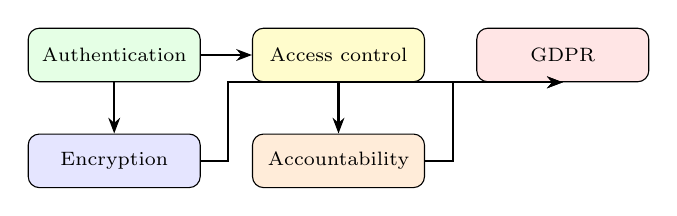
\begin{tikzpicture}[node distance=0.65cm]
    \node[lessonbox, fill=green!10] (authn) {Authentication};
    \node[lessonbox, right=of authn, fill=yellow!20] (authz) {Access control};
    \node[lessonbox, below=of authn, fill=blue!10] (crypto) {Encryption};
    \node[lessonbox, below=of authz, fill=orange!15] (audit) {Accountability};
    \node[lessonbox, right=of authz, fill=red!10] (gdpr) {GDPR};
    \draw[lessonarrow] (authn) -- (authz);
    \draw[lessonarrow] (authn) -- (crypto);
    \draw[lessonarrow] (authz) -- (audit);
    \draw[lessonarrow] (audit.east) -- ++(0.35,0) |- (gdpr.south);
    \draw[lessonarrow] (crypto.east) -- ++(0.35,0) |- (gdpr.south);
  \end{tikzpicture}
  \end{center}

  \vspace{0.35cm}
  \begin{block}{Reading the map}
    Authentication names the actor. Access control limits the actor. Encryption protects authentication material and sessions. Logging makes actions accountable. GDPR gives the hospital a legal reason to make all of this reliable.
  \end{block}
\end{frame}

\begin{frame}[c]{Final Recap}
  \begin{block}{Authentication foundations}
    Identification presents an identity; verification proves the claim. Authentication is not authorization, but authorization depends on it.
  \end{block}

  \begin{block}{Mechanisms}
    Passwords, tokens, smart cards, biometrics, challenge-response, and OTP all provide evidence, but each has different failure modes.
  \end{block}

  \begin{block}{Healthcare design lesson}
    Strong authentication must fit clinical reality: shared workstations, remote access, emergencies, usability pressure, audit needs, and sensitive patient data.
  \end{block}
\end{frame}

\begin{frame}[allowframebreaks]{References}
  \scriptsize
  \bibliographystyle{apalike-AMS}
  \bibliography{main}
\end{frame}

\end{document}
